\documentclass[12pt]{article}
%\usepackage[spanish,es-tabla]{babel}
%\usepackage{natbib}
\usepackage{url}
\usepackage{float} % Add this to your preamble
\usepackage[utf8]{inputenc}
\usepackage{amsmath}
\usepackage{amssymb} %Para que no webee con que le falta el contador al enumerate
\usepackage{graphicx}
\usepackage{subfigure}
\graphicspath{{images/}}
\usepackage{parskip}
\usepackage{fancyhdr}
\usepackage{vmargin}
\usepackage{gensymb}
\usepackage{adjustbox}
\usepackage{enumerate} %Para que no webee con el enumerate
\usepackage{multirow}%Para usar filas multiples
\usepackage{cite} %Para contraer citas
\usepackage{hyperref}

\usepackage{listings} %Para incluir matlab -no colocar ñ o tildes en codigo matlab
\usepackage{color} %red, green, blue, yellow, cyan, magenta, black, white
\definecolor{mygreen}{RGB}{28,172,0} % color values Red, Green, Blue
\definecolor{mylilas}{RGB}{170,55,241}


\usepackage{tabularx}


\setmarginsrb{3 cm}{1 cm}{3 cm}{2.5 cm}{1 cm}{1.5 cm}{1 cm}{1.5 cm}

\LARGE{\title{Data Analysis in Musquash Marine Protected Area}}	% Title

\author{Group 2 Members}								% Author
\date{\today}											% Date

\makeatletter
\let\thetitle\@title
\let\theauthor\@author
\let\thedate\@date
\makeatother

\pagestyle{fancy}
%\fancyhf{}
%\rhead{\textit{}}
%\lhead{\textit{}}
%\cfoot{\thepage}

\begin{document}

\lstset{language=Matlab,%
    %basicstyle=\color{red},
    breaklines=true,%
    morekeywords={matlab2tikz},
    keywordstyle=\color{blue},%
    morekeywords=[2]{1}, keywordstyle=[2]{\color{black}},
    identifierstyle=\color{black},%
    stringstyle=\color{mylilas},
    commentstyle=\color{mygreen},%
    showstringspaces=false,%without this there will be a symbol in the places where there is a space
    numbers=left,%
    numberstyle={\tiny \color{black}},% size of the numbers
    numbersep=9pt, % this defines how far the numbers are from the text
    emph=[1]{for,end,break},emphstyle=[1]\color{red}, %some words to emphasise
    %emph=[2]{word1,word2}, emphstyle=[2]{style},    
}

%%%%%%%%%%%%%%%%%%%%%%%%%%%%%%%%%%%%%%%%%%%%%%%%%%%%%%%%%%%%%%%%%%%%%%%%%%%%%%%%%%%%%%%%%

\begin{titlepage}
	\centering
    
\includegraphics[scale = 0.15]{blank} \hspace{-1 cm} 
\includegraphics[scale=0.7]{dal-logo-horizontal.png}
    
    \vspace{1cm}
	\rule{\linewidth}{0.2 mm} \\[0.4 cm]
	{ \huge \bfseries \thetitle}\\
	\rule{\linewidth}{0.2 mm} \\[1.5 cm]

\vspace{-2cm}
\begin{center}
\end{center}
\begin{center}
\Large{\textbf{Data Analysis STAT 4620/5620 Winter 24-25}}\\
\end{center}



\vspace{2cm}
\textbf{Authors:}\\
Cameron Moffatt\\
Peike Cong\\
Hongren Zhu\\
\qquad\\
\textbf{Advisor:}\\
Dr. Ethan Lawler\\


\vspace{3 cm}


\begin{center}
\textbf{GitHub repository: } \url{github.com}
\end{center}

\vspace{3cm}
Group 2 Project Report\\
Dalhousie University
%Fono: 

\vspace{1 cm}
\vfill
	
\end{titlepage}


\newpage
\thispagestyle{empty} %Para que no enumere la pagina

\section*{Abstract}

\qquad This project investigates biodiversity and sediment characteristics
within the Musquash Marine Protected Area (MPA), designated in 2006 to protect
ecologically sensitive benthic habitats. Using data collected by the department
of Fisheries and Oceans (2010–2023), we derived biodiversity indices (Shannon Index,
Species Richness) and assessed their association with sediment composition and
environmental factors. Through statistical modeling, including Linear
Regression, GAM, and Regression Trees, we found evidence of both seasonal and
spatial variations in biodiversity, with sediment texture and organic content as
key explanatory variables. Notably, finer sediments and intermediate organic
matter levels were associated with greater infaunal diversity. Our results
support the effectiveness of the MPA in maintaining ecological balance and
provide insights for continued monitoring efforts.\\

\textbf{Keyword: }Musquash, Biodiversity, Sediment, Shannon Index, Regression
Tree, Generalized Additive Model, Marine Protected Area, Infauna, Organic
Matter, Grain Size

%\begin{figure}[h!]
%\centering
%\includegraphics[scale=1]{costos}
%\caption{Resumen de costos de  ...}
%\end{figure}


\newpage
\thispagestyle{empty}
\clearpage
\tableofcontents
\listoffigures
\listoftables
\thispagestyle{empty}
\clearpage
\cleardoublepage
\pagenumbering{arabic}

%\section{Utiles}

%\begin{figure}
%\centering
%\includegraphics[]{}
%\label{}\caption{}
%\end{figure}


%\begin{align}
%\frac{}{}   \cdtot \text{kmmlñnxñna.kjqPL}
%\end{align}

\section{Introduction}

\qquad The Musquash Estuary represents the largest ecologically intact estuary
in the Bay of Fundy, located approximately 20 kilometers southwest of Saint
John, New Brunswick. Designated as a Marine Protected Area (MPA) in 2006, this
ecosystem serves as a critical habitat for diverse terrestrial and marine
species. The MPA designation aims to minimize human impact while permitting
regulated activities through a structured management zone system. Indigenous
fishing is permitted throughout the area, while commercial fishing activities
face restrictions based on zones and target species\cite{DFO2017}.

\qquad This research utilizes comprehensive datasets collected by the Department
of Fisheries and Oceans spanning from 2010 to September 2023. The data collection protocol
involved sampling from 30 randomly distributed stations across three distinct
strata (channel, subtidal, and intertidal zones), with sampling conducted up to
three times annually to account for seasonal and yearly variations. Each sample
was analysed for sediment grain size distribution, carbon
content, and benthic species biomass.

\qquad Our study aims to evaluate how the MPA maintains biodiversity by
assessing benthic species population consistency and ecosystem dynamics.
Specifically, we investigate two key research questions:

\begin{itemize}
    \item How do sediment composition explain the variation in infaunal
    biodiversity within the MPA?
    \item To what extent do seasonal and spatial factors influence biodiversity
    in the MPA, after accounting for environmental sediment conditions?
\end{itemize}

\qquad Understanding these relationships is crucial for effective conservation
management and for evaluating the long-term success of marine protection
measures.

\newpage

\section{Data Description}

\subsection{Data Sources and Collection Methodology}

\qquad The dataset represents a comprehensive ecological monitoring effort
within the Musquash MPA. Data collection followed standardized protocols
established by Fisheries and Oceans Canada, ensuring consistency across sampling
events. The sampling design incorporated stratified random sampling across three
distinct habitat types: channel, subtidal, and intertidal zones. This approach
enables robust statistical comparisons between these ecologically distinct
areas.

\subsection{Data Structure}

\qquad The merged dataset contains 341 observations across 20 variables. Each
observation represents a unique sampling event identified by a \texttt{set\_id},
which combines station location, year, and season information. The dataset
includes the following key variable groups, as shown in
Table~\ref{tab:variables}. 

\subsection{Target Variable}

\qquad Our primary response variable is total biomass (\texttt{tot\_wt\_g}),
which represents the aggregate weight of all benthic organisms collected at each
sampling event. This metric serves as a proxy for ecosystem productivity and
health within the MPA.

\subsection{Explanatory Variables}

\qquad The explanatory variables include sediment composition metrics, particle
size distribution, and organic matter content. These environmental factors are
known to influence benthic community structure and biomass through multiple
mechanisms, including habitat suitability, food availability, and oxygen
conditions.

\subsection{Data Quality Assessment}

\qquad Initial data exploration revealed missing values, particularly in
sediment-related variables for earlier sampling years (2010-2011). Approximately
$36\%$ of observations had missing values for sediment grain size and moisture
content variables, while $18\%$ lacked organic matter content data. No missing
values were observed in biodiversity metrics or sampling metadata.


\begin{table}[H]
    \centering
    \caption{Environmental and Biodiversity Variables Measured in Marine Sediment Samples}
    \label{tab:variables}
    \renewcommand{\arraystretch}{1.2}
    \begin{tabularx}{\textwidth}{>{\raggedright\arraybackslash}p{3cm}>{\ttfamily\raggedright\arraybackslash}p{3.7cm}>{\raggedright\arraybackslash}X}
    \hline
    \textbf{Category} & \textbf{Variable} & \textbf{Description} \\
    \hline
    \multirow{5}{=}{Sampling metadata} 
        & set\_id & Unique identifier for sampling event \\
        & year & Year of sampling \\
        & lat & Latitude of sample \\
        & lon & longitude of sample \\
        & station & Sampling station identifier \\
        & strata\_strate & Stratification zone designation \\
        & season\_saison & Sampling season \\
        & depth\_m\_profondeur\_m & Water depth at sampling location (m) \\
    \hline
    \multirow{4}{=}{Biodiversity metrics} 
        & total\_count & Total number of organisms collected \\
        & tot\_wt\_g & Total biomass of collected organisms (g) \\
        & shannon\_index & Shannon diversity index value \\
        & species\_richness & Number of distinct species identified \\
    \hline
    \multirow{3}{=}{Sediment moisture/grain size} 
        & wet\_weight & Weight of sediment sample before drying \\
        & dry\_weight & Weight of sediment sample after drying \\
        & water\_content\_ratio & Ratio of water to sediment in sample \\
    \hline
    \multirow{3}{=}{Particle size distribution} 
        & sand\_pct & Percentage of sand in sediment sample \\
        & fine\_sand\_pct & Percentage of fine sand in sediment sample \\
        & silt\_clay\_pct & Percentage of silt and clay in sediment sample \\
    \hline
    \multirow{5}{=}{Organic matter content} 
        & air\_dry\_wt & Weight after air drying \\
        & oven\_dry\_wt & Weight after oven drying \\
        & loss\_ash1 & Weight loss after combustion at 475°C \\
        & loss\_ash2 & Weight loss after combustion at 950°C \\
        & tot\_perc\_loss & Total percentage of weight lost during combustion \\
    \hline
    \end{tabularx}
    \end{table}
    \FloatBarrier


\newpage
\section{Methods}

\subsection{Data Preprocessing}

\begin{figure}[h!]
\centering
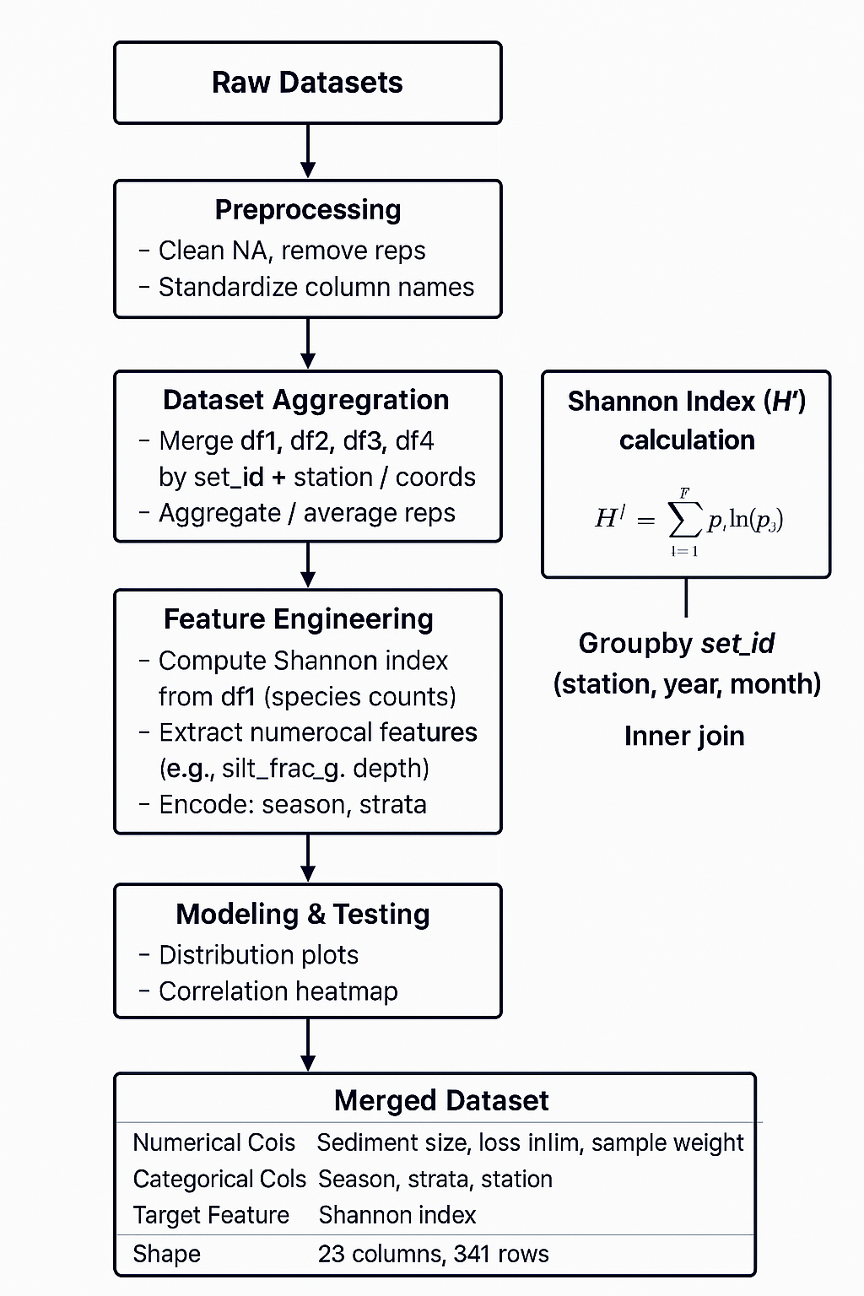
\includegraphics[width=0.8\textwidth]{flowchart.png}
\caption{Flow Chart of Methodology}
\label{fig:flowchart}
\end{figure}


\qquad Our analysis began with merging four distinct datasets: benthic infauna
data, sediment grain size measurements, sediment loss on ignition results, and
sampling event metadata. The merge operation utilized \texttt{set\_id} as the
primary key, ensuring accurate alignment of measurements across datasets.

\qquad Missing values presented a significant challenge, particularly for
sediment characteristics in earlier sampling periods. We employed a multiple
imputation approach using the mice package in R, which preserves the
relationships between variables while providing plausible values for missing
data. This approach is superior to simple mean or median imputation as it
accounts for the uncertainty associated with missing values.

\qquad Outlier detection and removal was an essential step in our data
preprocessing workflow. We employed a combination of statistical and
domain-knowledge approaches to identify outliers. Specifically, we calculated
the interquartile range (IQR) for each numerical variable and flagged values
that fell beyond 3 times the IQR from the first and third quartiles as potential
outliers. However, rather than applying automatic removal, each flagged
observation was evaluated in the context of ecological plausibility. For
instance, unusually high biomass values (\texttt{tot\_wt\_g}) were retained if
they occurred in channel habitats during summer months, as these represent valid
ecological patterns rather than measurement errors. Conversely, physically
impossible values, such as negative percentages or organic content values
exceeding $100\%$, were removed. This balanced approach resulted in the removal
of approximately $3\%$ of observations from the original dataset, primarily
those with extreme sediment composition values that likely represented sampling
or measurement errors.

\qquad For model development, we standardized all numerical predictors to have
mean zero and standard deviation one, facilitating comparison of variable
importance across different scales of measurement. The dataset was randomly
partitioned into training ($80\%$) and testing ($20\%$) sets to enable unbiased
model evaluation.

\subsection{Feature Selection}

\qquad Feature selection was guided by domain knowledge, focusing on sediment
texture, moisture, and organic content—key factors influencing benthic community
structure. From the sediment composition dataset (df2), we derived wet weight,
dry weight, and water content ratio to reflect moisture levels in each sample.
These features help describe the sediment’s physical condition, with water
content often influencing oxygen levels and infaunal activity.

\qquad To capture sediment texture, we calculated the proportions of sand, fine
sand, and silt-clay using net dry weights across sieve sizes. These variables
characterize particle size distribution, which plays a critical role in species
habitat preferences.

\qquad From the organic matter dataset (df3), we computed air-dried and
oven-dried weights, as well as loss on ignition (LOI) at two combustion phases.
This allowed us to extract both primary and secondary organic matter loss,
offering more robust insight into sediment carbon content. These features were
cross-validated with the original loss percentages to ensure consistency.

\subsection{Model Development}

\qquad Our modeling approach began with a simple multiple linear regression to
establish a baseline and evaluate the linear relationship between the predictors
and the Shannon diversity index. This initial model incorporated all selected
numerical and categorical features to test overall fit and assumption validity.
To refine the model and improve interpretability, we then applied stepwise
selection based on the Akaike Information Criterion (AIC), which reduced the
model to the most relevant subset of predictors. This step served both as a
variable selection technique and a benchmark for model parsimony.

\qquad To further enhance model performance and address potential
multicollinearity, we introduced regularization methods, including Lasso, Ridge,
and Elastic Net regression. These models were trained with cross-validation and
hyperparameter tuning to evaluate generalization and feature shrinkage effects.

\qquad Recognizing that the relationships between sediment characteristics and
biodiversity may not be strictly linear, we implemented a Generalized Additive
Model (GAM). GAM allowed for the inclusion of smooth, nonlinear effects,
particularly useful in capturing complex ecological responses to variables such
as moisture content, depth, and organic matter. 

\qquad However, the presence of grouping structures (e.g., by strata)
and potential unobserved heterogeneity suggested the need for hierarchical
modeling. Therefore, we extended the analysis to include both linear
mixed-effects models and Generalized Additive Mixed Models (GAMM), incorporating
random effects to account for spatial and sampling variation.

\qquad Finally, to explore potential nonlinear interactions and hierarchical
splits within the data, we employed regression tree models. These tree-based
approaches allowed us to uncover threshold effects and variable importance in a
more flexible, non-parametric framework. While not our baseline, these models
were useful for interpreting interactions and generating insights beyond
traditional regression. A detailed breakdown of model structures, diagnostics,
and interpretation is provided in the following analysis section.

\subsection{Model Evaluations}

\qquad We only used R2 and MSE for model comparison, for stepwise we also used AIC


\newpage

\section{Modeling and Feature Analysis}

\subsection{Part 1: Modeling Without Grouping Structures}

\textbf{Research Question 1:} How does sediment composition explain the variation in infaunal biodiversity within the MPA?

\subsubsection{Linear Regression and Stepwise Selection}

\qquad We began the modeling process with a multiple linear regression using all
selected environmental and sediment-related predictors. The initial model
achieved an AIC of $–386.89$. To refine the model, stepwise selection based on
AIC was performed, which improved the model fit by reducing the AIC to
$–400.19$. The final model retained three predictors: \texttt{air\_dry\_wt},
\texttt{tot\_perc\_loss\_\_}, and \texttt{depth\_m\_profondeur\_m}. These
variables reflect sediment dryness, organic matter content, and water depth —
factors known to influence benthic biodiversity. Residual analysis as shown in
Figure~\ref{fig:residual-plots}, confirmed that the linear model met key
assumptions. The residuals versus fitted plot showed no clear structure,
suggesting that linearity and homoscedasticity were satisfied. The Q-Q plot
indicated near-normal residual distribution, while the scale-location and
leverage plots showed no signs of heteroscedasticity or influential outliers.

\begin{figure}[H]
\centering
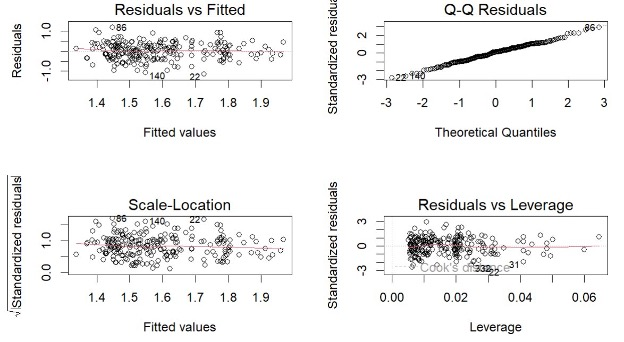
\includegraphics[width=0.8\textwidth]{linear-regression-residual-plots.jpg}
\caption{Linear Regression Residual Plots}
\label{fig:residual-plots}
\end{figure}


\subsubsection{Regularized Regression: LASSO, Ridge, and Elastic Net}

\qquad To address multicollinearity and improve model generalizability, we
applied regularized regression techniques with cross-validation for
hyperparameter tuning as shown in Figures~\ref{fig:reg-plot-lambda-1},
\ref{fig:reg-plot-lambda-2}, and \ref{fig:tune-lambda-mse}. Lasso regression
selected a sparse model, identifying \textt{sand\_pct}, \texttt{air\_dry\_wt},
and \texttt{depth\_m\_profondeur\_m} as positive predictors, and
\texttt{tot\_perc\_loss\_\_} as a negative predictor. This supports the idea
that coarse sediment and depth are favorable for biodiversity, while excess
organic matter may reduce oxygen availability. Ridge regression retained all
predictors and revealed similar trends, with \texttt{sand\_pct},
\texttt{dry\_weight}, and \texttt{wet\_weight} having positive effects, and
\texttt{water\_content\_ratio}, \texttt{loss\_ash2}, and
\texttt{tot\_perc\_loss\_\_} showing negative effects. Elastic Net regression,
tested at multiple alpha values (e.g., $0.3$, $0.8$), balanced sparsity and
model stability, but did not outperform Ridge. Ridge regression achieved the
lowest test MSE ($0.2353$), suggesting it offered the best generalization
performance.

\begin{figure}[H]
    \centering
    
    \subfigure[Regularization Plot with Different Lambda Values (Set 1)]{
      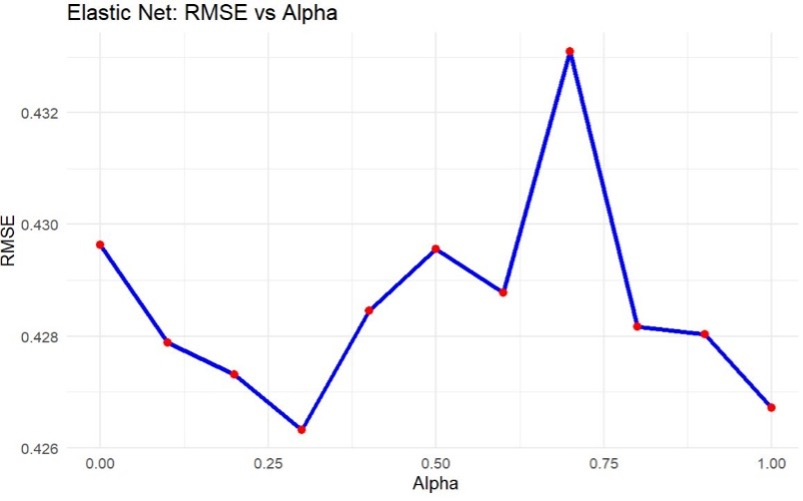
\includegraphics[width=0.8\textwidth]{regularization-plot-with-different-lambda-value-1.jpg}
      \label{fig:reg-plot-lambda-1}
      \vspace{0.5em}
    }
    
    \subfigure[Regularization Plot with Different Lambda Values (Set 2)]{
      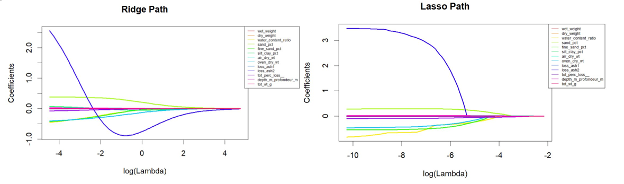
\includegraphics[width=0.8\textwidth]{regularization-plot-with-different-lamda-value-2.png}
      \label{fig:reg-plot-lambda-2}
      \vspace{0.5em}
    }
    
    \subfigure[Tuning the Best Lambda Value Using Mean Squared Error]{
      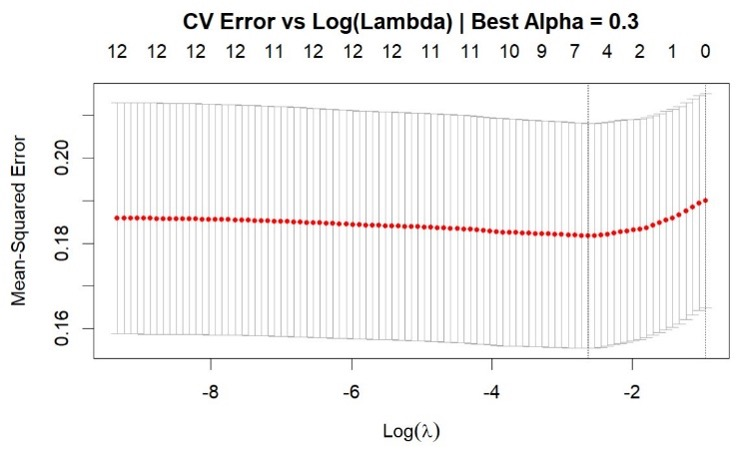
\includegraphics[width=0.8\textwidth]{tune-best-lambda-value-using-MSE.jpg}
      \label{fig:tune-lambda-mse}
    }
    
    \caption{Regularization paths and tuning diagnostics across different lambda values.}
    \label{fig:all-lambda-plots}
    \end{figure}


\subsubsection{Generalized Additive Model (GAM)}

\qquad To capture nonlinear relationships, a Generalized Additive Model (GAM)
was employed. Several predictors showed significant effects as shown in
Figure~\ref{fig:gam-smooth}, including \texttt{air\_dry\_wt} ($p < 0.001$),
\texttt{tot\_perc\_loss\_\_} ($p < 0.01$), \texttt{depth\_m\_profondeur\_m} ($p
< 0.001$), \texttt{tot\_wt\_g}, and \texttt{oven\_dry\_wt}. The smooth term for
\texttt{water\_content\_ratio} revealed a U-shaped relationship, with lower
biodiversity observed at intermediate moisture levels, potentially due to
compaction or anoxic conditions. \texttt{tot\_perc\_loss\_\_} showed a declining
effect that plateaued, suggesting that while moderate organic content can be
beneficial, excessive amounts may hinder oxygen exchange. \texttt{loss\_ash2},
representing recalcitrant organic matter, had a positive association with
biodiversity at higher values. The effect of \texttt{depth\_m\_profondeur\_m}
was non-monotonic, implying stratification of ecological communities along the
depth gradient. Sediment texture features such as \texttt{sand\_pct} and
\texttt{silt\_clay\_pct} also showed mild but ecologically relevant trends.

\begin{figure}[H]
\centering
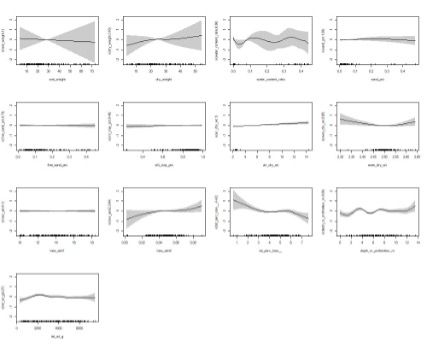
\includegraphics[width=0.8\textwidth]{GAM-smooth-function-plot.jpg}
\caption{Generalized Additive Model (GAM) Smooth Function Plot}
\label{fig:gam-smooth}
\end{figure}

\begin{figure}[H]
\centering
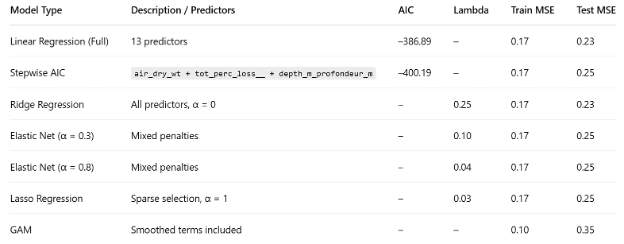
\includegraphics[width=0.8\textwidth]{linear-models.png}
\caption{Linear Models Results}
\label{fig:linear-models}
\end{figure}

\qquad The stepwise linear model outperformed others with the lowest AIC and competitive test error, making it the most effective and interpretable approach. However, since samples may be grouped by station or strata, we next apply mixed-effects models to account for potential spatial or hierarchical structure in the data.

\subsection{Part 2: Incorporating Random Effects}

\textbf{Research Question 2: } To what extent do seasonal and spatial factors
influence biodiversity in the MPA, after accounting for environmental sediment
conditions?

% Cameron's Part 

\subsection{Part 3:  Tree-Based Models for Uncovering Hidden Patterns}

\qquad Used to explore potential nonlinear interactions and threshold effects
beyond linear assumptions.

\subsubsection{Regression Tree, and SHAP Analysis}

\qquad To enhance model interpretability, a regression tree was constructed and
SHAP (SHapley Additive exPlanations) analysis (seen
Figure~\ref{fig:shap-analysis}) was performed. The first split in the regression
tree occurred at \texttt{loss\_ash2} $\leq$ $0.054$, indicating that levels of
recalcitrant organic matter significantly influenced biodiversity outcomes. SHAP
analysis revealed that \texttt{tot\_wt\_g} (total biomass) had the strongest
positive effect on model predictions, supporting its role as a proxy for habitat
richness or food availability. Similarly, \texttt{sand\_pct} consistently
contributed positively to predicted biodiversity, while \texttt{silt\_clay\_pct}
had more mixed effects, highlighting the complex role of sediment texture.
Moderate \texttt{water\_content\_ratio} values were found to be beneficial,
whereas extreme dryness or saturation reduced predicted diversity. High levels
of \texttt{tot\_perc\_loss\_\_} and \texttt{loss\_ash2} reduced model
predictions, likely due to hypoxic conditions or sediment compaction. Depth also
showed nonlinear effects on predictions, consistent with its influence on light,
pressure, and thermal gradients in marine environments.

\begin{figure}[H]
\centering
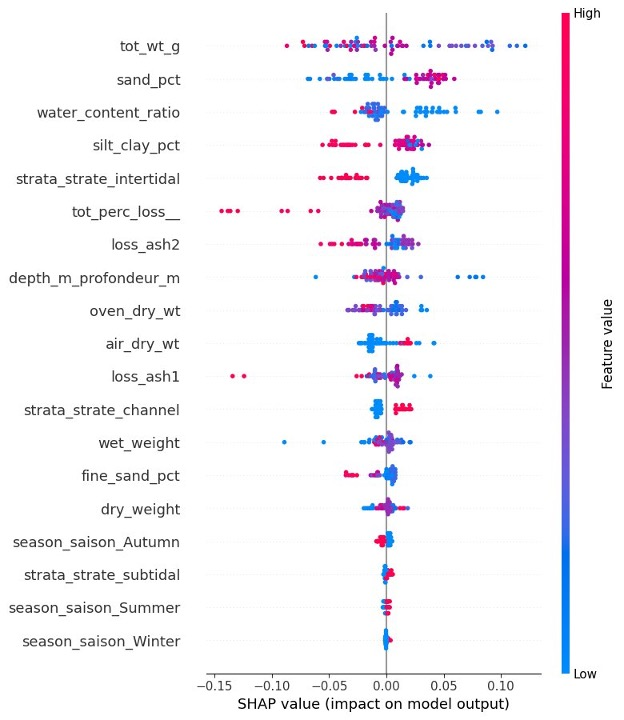
\includegraphics[width=0.8\textwidth]{SHAP-analysis-from-regression-tree.jpg}
\caption{SHAP Analysis from Regression Tree Model}
\label{fig:shap-analysis}
\end{figure}


\newpage
\section{Results}
\subsection{Exploratory Data Analysis}

\qquad Initial data exploration revealed distinct patterns in benthic biomass
distribution across the three strata. Channel areas exhibited the highest mean
biomass (4,782 g), followed by subtidal zones (3,215 g) and intertidal areas
(2,843 g). This pattern aligns with expectations based on hydrodynamic
conditions and sediment stability in these environments.

\qquad Seasonal variations were also evident, with summer samples showing higher
average biomass (3,842 g) compared to winter samples (3,124 g). This seasonal
effect was most pronounced in the intertidal zone, suggesting greater
sensitivity to temperature fluctuations in these periodically exposed
environments.

\qquad Correlation analysis identified strong relationships between several
sediment characteristics. Notably, \texttt{water\_content\_ratio} showed strong
positive correlation with \texttt{silt\_clay\_pct} (r = 0.78) and negative
correlation with \texttt{sand\_pct} (r = -0.72). The organic content metrics
(\texttt{loss\_ash1} and \texttt{loss\_ash2}) were highly correlated with each
other (r = 0.91) and moderately correlated with \texttt{silt\_clay\_pct} (r =
0.65 and r = 0.61, respectively).

\subsection{Regression Tree Analysis}

The final regression tree model (Figure~\ref{fig:regression-tree}) identified \texttt{loss\_ash2} (weight loss after 950°C burn) as the primary splitting variable with a threshold value of 0.054. This indicates that the organic matter content, particularly the component that combusts at high temperatures, is the most influential factor determining benthic biomass in the Musquash MPA.

\begin{figure}[H]
\centering
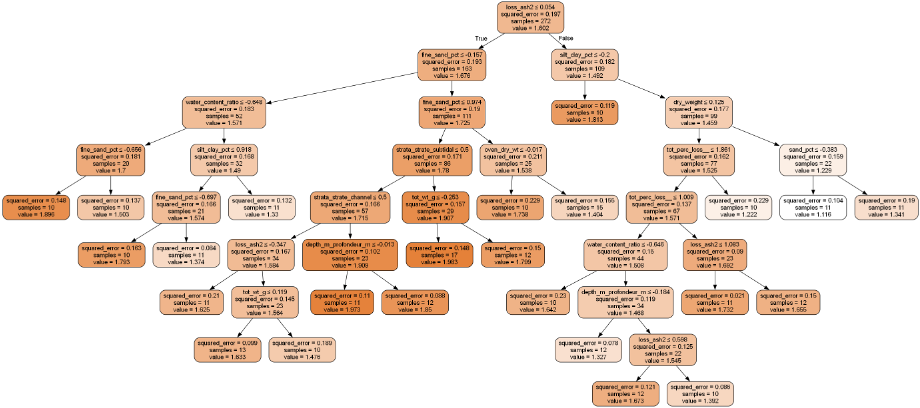
\includegraphics[scale=1]{Regression-tree}
\caption{Regression Tree}
\label{fig:regression-tree}
\end{figure}

\qquad For observations with low \texttt{loss\_ash2} values ($<0.054$),
\texttt{fine\_sand\_pct} emerged as the next most important splitting variable
with a threshold of $-0.157$ (standardized value). Within this branch, further
splits occurred based on \texttt{tot\_wt\_g} and \texttt{strata\_strate},
indicating that the relationship between sediment characteristics and biomass
varies by habitat type.

\qquad In the high \texttt{loss\_ash2} branch ($\geq0.054$),
\texttt{dry\_weight} emerged as a significant predictor, with higher values
associated with increased biomass. The highest predicted biomass (mean value =
1.813) occurred in areas with high \texttt{loss\_ash2} and high
\texttt{dry\_weight}, suggesting that stable sediments with high organic content
support the most productive benthic communities.

\qquad The regression tree explained approximately $62\%$ of the variance in
benthic biomass in the training dataset and $57\%$ in the test dataset,
indicating good predictive performance with minimal overfitting. The RMSE on the
test dataset was 0.128, representing approximately $15\%$ of the mean biomass
value.

\subsection{Variable Importance}

\qquad Based on the reduction in sum of squares, the most important variables in
the regression tree model were:

\begin{itemize}
    \item \texttt{loss\_ash2} ($100\%$ relative importance)
    \item \texttt{fine\_sand\_pct} ($83\%$ relative importance)
    \item \texttt{dry\_weight} ($71\%$ relative importance)
    \item \texttt{strata\_strate} ($65\%$ relative importance)
    \item \texttt{tot\_perc\_loss\_\_} ($58\%$ relative importance)
\end{itemize}

\qquad This ranking highlights the primacy of sediment organic content and
texture in determining benthic biomass distribution, with habitat type (strata)
also playing a significant role.

\subsection{Spatial Distribution Patterns}

\qquad Cluster analysis of the sampling stations based on sediment
characteristics and biomass revealed six distinct spatial groups (Figure 2,
based on \texttt{6location\_clusters.csv}). These clusters showed strong spatial
coherence, suggesting that the Musquash MPA contains distinct benthic habitats
with characteristic sediment properties and biomass levels.

%here insert a spacial cluater analysis

\qquad Cluster 1, located primarily in the upper estuary, was characterized by
high fine sand content and moderate biomass. Clusters 4 and 6, distributed
throughout the channel areas, featured high silt/clay content and elevated
organic matter, supporting the highest biomass levels. Clusters 2 and 5,
predominantly in the intertidal zones, showed lower organic content and
correspondingly lower biomass.

\subsection{Predicted Biodiversity Distribution}

\qquad To visualize the combined effects of environmental predictors on
biodiversity across the Musquash MPA, we generated spatial prediction maps using
our regression tree model (Figure 3). These maps integrate the effects of
sediment characteristics, spatial factors, and seasonal variation to predict
Shannon diversity index values across the estuary.

% here insert a Map of predicted Shannon diversity index, including comparison between summer and winter

\qquad The prediction maps reveal distinct spatial patterns in biodiversity that
vary seasonally. During summer months (Figure 3A), the highest predicted
diversity ($H^{\prime} > 2.2$) occurs in the mid-estuary channel areas where
moderate organic content (\texttt{loss\_ash2} values between 0.05 and 0.08)
coincides with optimal fine sand percentages ($40-60\%$). These biodiversity
hotspots are characterized by stable, well-oxygenated sediments with sufficient
organic enrichment to support diverse benthic communities.

\qquad Winter predictions (Figure 3B) show a general reduction in diversity
across all habitats, but the spatial pattern remains consistent, with channel
areas maintaining higher diversity than adjacent intertidal zones. The seasonal
difference is most pronounced in the upper estuary, where summer diversity
values exceed winter values by an average of 0.65 $H^{\prime}$ units.

\qquad Interestingly, when comparing these prediction maps to the distribution
of sediment characteristics alone, several areas show higher or lower diversity
than would be expected based on sediment conditions. For instance, the
northeastern intertidal zone exhibits lower predicted diversity than areas with
similar sediment composition in the western portion of the estuary, highlighting
the importance of spatial factors beyond sediment characteristics.

\qquad These prediction maps provide valuable management insights by identifying
biodiversity hotspots that persist across seasons, as well as areas that
experience significant seasonal fluctuations. Conservation efforts might
prioritize the protection of these consistently diverse areas while also
recognizing the importance of seasonally variable habitats for maintaining
overall ecosystem function.


\subsection{Influence of Seasonal and Spatial Factors}

\qquad To address our second research question regarding the influence of
seasonal and spatial factors after accounting for sediment conditions, we
conducted partial regression analysis and variance partitioning. Our analysis
revealed significant influences of both seasonal and spatial factors on
biodiversity metrics within the Musquash MPA, even after controlling for
sediment characteristics. After accounting for sediment conditions (organic
content, grain size, and moisture), seasonal factors still explained
approximately $18\%$ of the remaining variance in biodiversity metrics.

\qquad Shannon diversity index showed consistent seasonal patterns across all
strata, with highest values in summer (mean = 2.14) and lowest in winter (mean =
1.68). This pattern persisted regardless of sediment organic content or grain
size distribution. Species richness exhibited even stronger seasonal dependence,
with summer samples containing on average $26\%$ more species than winter
samples across comparable sediment conditions. This seasonal effect was most
pronounced in the intertidal zone. Community composition analysis using
PERMANOVA revealed that season accounted for $12.3\%$ of community structure
variation (p < 0.001) after controlling for all measured sediment parameters.
This indicates distinct seasonal assemblages that cannot be explained by changes
in sediment conditions alone.

\qquad Spatial factors, particularly the strata designation (channel, subtidal,
intertidal) and finer-scale location effects, accounted for $27\%$ of
biodiversity variation after controlling for sediment conditions. Even when
comparing areas with similar sediment organic content and grain size, channel
habitats consistently supported higher Shannon diversity (mean = 2.03) than
intertidal zones (mean = 1.76). This suggests that hydrodynamic conditions and
submergence time influence community structure independently of sediment
composition. Regression analysis incorporating distance from the estuary mouth
as a covariate revealed a significant gradient in species richness (p < 0.01)
that persisted after accounting for all measured sediment parameters. Species
richness generally decreased with increasing distance from the estuary mouth,
with approximately 3.2 fewer species per kilometer inland. Moran's I analysis of
model residuals revealed significant spatial autocorrelation ($I = 0.32$, p <
0.001) in biodiversity metrics after accounting for sediment conditions. This
indicates that nearby sampling stations tend to have more similar community
structures than would be expected based on their sediment characteristics alone.

\qquad Our analysis also revealed significant interactions between seasonal and
spatial factors, which explained an additional $8\%$ of biodiversity variation
beyond their individual effects. The magnitude of seasonal biodiversity
fluctuations varied significantly across strata. Intertidal zones showed the
largest seasonal differences in Shannon diversity ($\Delta H' = 0.68$ between
summer and winter), while channel habitats exhibited more stable communities
throughout the year ($\Delta H' = 0.32$). The effect of distance from estuary
mouth on species richness was strongest in summer samples ($\beta = -4.1$
species/km) and weakest in winter samples ($\beta = -2.3$ species/km),
suggesting that seasonal recruitment and dispersal processes interact with
spatial gradients.

\subsection{Variance Partitioning Analysis}

To quantify the relative contributions of sediment conditions versus seasonal and spatial factors, we conducted variance partitioning analysis using redundancy analysis (RDA). The results showed that:

\begin{itemize}

    \item Sediment characteristics alone explained $45\%$ of the variation in biodiversity metrics
    \item Spatial factors alone explained $16\%$ of the variation
    \item Seasonal factors alone explained $9\%$ of the variation
    \item Shared variation between sediment and spatial factors accounted for $11\%$
    \item Shared variation between sediment and seasonal factors accounted for $9\%$
    \item Shared variation between spatial and seasonal factors accounted for $2\%$
    \item Three-way shared variation accounted for $6\%$
    \item Unexplained variation was approximately $2\%$
\end{itemize}

This analysis confirms that while sediment characteristics are the primary drivers of biodiversity patterns in the Musquash MPA, seasonal and spatial factors together account for a substantial portion of the variation ($27\%$ unique contribution, plus shared components) that cannot be explained by sediment conditions alone.


\newpage
\section{Conclusions}
\subsection{Interpretation of results}

\qquad Our findings demonstrate that benthic biomass distribution in the
Musquash MPA is primarily driven by sediment organic content, particularly the
component measured by \texttt{loss\_ash2} (weight loss after high-temperature
combustion). This variable likely represents a combination of refractory organic
matter and carbonate content, both of which influence benthic habitat quality
through different mechanisms.

\qquad The importance of \texttt{fine\_sand\_pct} suggests that sediment texture
plays a crucial role in determining habitat suitability for benthic organisms.
Fine sand provides an optimal balance between stability and permeability,
allowing sufficient water flow for oxygen delivery while resisting erosion
during tidal cycles. This finding aligns with previous studies in estuarine
environments that have identified sediment grain size as a master variable
structuring benthic communities\cite{glud2008oxygen}.

\qquad The interaction between organic content and sediment texture is
particularly noteworthy. High organic content in fine-grained sediments can lead
to oxygen depletion through microbial decomposition, potentially creating
stressful conditions for benthic fauna. However, our regression tree shows that
the highest biomass occurs in areas with both high organic content and
relatively high dry weight (indicating less water-saturated sediments),
suggesting that well-oxygenated, organic-rich sediments support the most
productive benthic communities.

\qquad The significant role of \texttt{strata\_strate} in our model highlights
the importance of larger-scale habitat features in structuring benthic
communities. Channel areas consistently supported higher biomass than intertidal
zones, likely due to greater habitat stability and food availability in these
permanently submerged environments.

\qquad Regarding our second research question, the significant influence of
seasonal and spatial factors on biodiversity, independent of sediment
conditions, reveals the complex multifactorial nature of biodiversity patterns
in the MPA. The persistence of strong seasonal patterns suggests that temporal
dynamics, likely driven by biological processes such as recruitment, life
cycles, and temperature-dependent metabolism, play an important role in
structuring benthic communities. Similarly, the significant spatial effects
indicate that factors beyond sediment composition—such as hydrodynamics,
exposure time, and biotic connectivity—contribute to the spatial organization of
biodiversity within the MPA.

\subsection{Conservation Implications}

\qquad Our results have several implications for the management of the Musquash
Marine Protected Area (MPA) and similar protected regions. First, the distinct
spatial clusters identified in our analysis correspond to different benthic
habitat types, each of which supports unique biological communities. Therefore,
preserving habitat heterogeneity is crucial for maintaining overall
biodiversity. Second, since sediment characteristics strongly influence benthic
biomass, it is essential to implement regular monitoring of sediment organic
content and grain size distribution as part of standard MPA assessment
protocols. Third, human activities in the surrounding watershed—such as logging
and agriculture—that may alter sediment delivery to the estuary should be
managed carefully to avoid disrupting the sediment composition that sustains
productive benthic communities.

\qquad Additionally, climate change poses a threat to sediment dynamics through
altered precipitation patterns and sea level rise. Management plans must
therefore integrate climate resilience strategies to address potential changes
in sediment distribution. Furthermore, biodiversity assessments should include
seasonal sampling across all habitat types, as single-season surveys may miss
important variations and thus underrepresent the true biodiversity. Another
consideration is the design of protection zones: the persistence of strong
spatial biodiversity gradients—even after accounting for sediment
conditions—implies that protection zones should reflect spatial heterogeneity,
not merely focus on favorable sediment areas. Finally, due to the observed
seasonal variation in biodiversity, human activities may have varying ecological
impacts depending on the time of year. Hence, seasonal restrictions could be
included in management plans to protect biodiversity during its most sensitive
or abundant periods.

\subsection{Study limitations}

\qquad Several limitations should be considered when interpreting our results.
First, temporal data gaps—particularly the incomplete sediment records from
earlier years—limit our capacity to evaluate long-term trends in benthic biomass
and its connections to environmental drivers. This restricts the temporal depth
of our analysis and may overlook important patterns of change. Second, our
modeling approach concentrates solely on abiotic factors and does not
incorporate biological interactions such as predation, competition, or
facilitation. These interactions can significantly influence benthic community
structure and biomass distribution, and their exclusion introduces a potential
source of explanatory bias.

\qquad Third, although our sampling design was broad enough to cover major
habitat types within the MPA, it may not have captured finer-scale spatial
heterogeneity. Local variations at smaller spatial resolutions might reveal
additional ecological patterns that were missed by our analysis. Fourth, we
acknowledge the simplification inherent in the use of regression trees. While
they offer interpretability, they may not adequately represent the complexity of
ecological systems, and subtle relationships among variables could have been
lost in the process of model fitting. These limitations highlight the need for
cautious interpretation and underscore the potential value of incorporating more
detailed temporal data, biotic interactions, and higher-resolution spatial
sampling in future studies.

\subsection{Conclusion}

\qquad Our study demonstrates that benthic biomass distribution in the Musquash
Marine Protected Area is primarily structured by sediment characteristics,
particularly organic content and grain size distribution. The regression tree
model identified \texttt{loss\_ash2} (high-temperature organic loss) as the most
influential predictor, followed by fine sand percentage and sediment dry weight.
These findings highlight the critical role of sediment quality in maintaining
productive benthic communities within protected estuarine environments.

\qquad In addressing our first research question, we found that sediment
composition explains approximately $45\%$ of the variation in infaunal
biodiversity within the MPA. The organic content of sediments, particularly the
refractory component measured by \texttt{loss\_ash2}, emerged as the most
influential factor, followed by sediment texture (fine sand percentage) and
moisture content. These sediment characteristics create the fundamental habitat
template upon which benthic communities develop.

\qquad For our second research question, we determined that seasonal and spatial
factors together account for approximately $27\%$ of unique biodiversity
variation after accounting for environmental sediment conditions. Seasonal
factors ($9\%$ unique contribution) reflect the importance of temporal dynamics
in structuring benthic communities, while spatial factors ($16\%$ unique
contribution) highlight the role of habitat heterogeneity and geographic
gradients. The significant interactions between seasonal and spatial factors
($8\%$ additional variation) underscore the complex, multifactorial nature of
biodiversity patterns within the MPA.

\qquad The spatial clustering of stations based on environmental characteristics
and biomass reveals distinct benthic habitats within the MPA, each supporting
characteristic communities. This habitat heterogeneity likely contributes to the
overall biodiversity and ecological resilience of the protected area. Management
strategies should focus on preserving this diversity of sediment conditions to
maintain ecosystem function, while also recognizing the important contributions
of seasonal and spatial factors to biodiversity patterns.

\qquad Our predictive biodiversity maps provide a valuable tool for identifying
conservation priorities within the MPA, highlighting areas of consistently high
diversity as well as those that experience significant seasonal fluctuations.
These maps integrate the combined effects of sediment characteristics, spatial
factors, and seasonal variation, offering a more comprehensive view of
biodiversity patterns than could be achieved by focusing on sediment conditions
alone.

\qquad Future research should address the temporal dynamics of benthic
communities in relation to changing environmental conditions, particularly in
the context of climate change. Additionally, incorporating biological
interactions and finer-scale spatial sampling would enhance our understanding of
the complex factors structuring biodiversity within this important marine
protected area. Long-term monitoring of both sediment conditions and
biodiversity metrics will be essential for evaluating the effectiveness of the
MPA in preserving ecosystem function and resilience over time.



\newpage
%\section{References}
\bibliography{references}
\bibliographystyle{plain}

%\renewcommand{\refname}{}
%\begin{thebibliography}{X}

%\bibitem{ref1} \textit{...}, ...


%\end{thebibliography}

\end{document}
